\newpage
\section{Probabilistic Model}

%----------------------------------------
\subsection{Basic Idea of Probabilistic Model}

\begin{itemize}
\item Probabilistic models ranking function: 
\begin{equation*}
f(d, q) = p(R=1 \,\big|\, d,q), \; R \in \{0,1\}
\end{equation*}
\item \textbf{Query Likelihood}: if a user likes document d, how likely would the user enter query q (in order to retrieve d)? 
\item Assumption: a user formulates a query based on an <<imaginary relevant document>>:
\begin{equation*}
p(R=1 \,\big|\, d,q) \approx p(q \,\big|\, d,R=1)
\end{equation*}
\item Basic idea based on user clicks (R=1):
\begin{equation*}
f(q, d) = p(R=1 \,\big|\, d,q) = \frac{count(q, d, R=1)}{count(q,d)}
\end{equation*}
\item How to compute $p(q \,|\, d)$? How to compute probability of
text in general? $\to$ \textbf{Language Model}
\end{itemize}


%----------------------------------------
\subsection{Language Model}
The term language model (LM) refers to a probabilistic model of text (i.e., it defines a probability distribution over sequences of words). 

Uses of a Language Model:
\begin{itemize}
\item Representing topics
\item Discovering word associations
\end{itemize}


%----------------------------------------
\subsection{The Simplest Language Model: Unigram LM}
Unigram Language Model = word distribution
\begin{itemize}
\item Generate text by generating each word \textbf{independently} 
\item Thus, $p(w_1, w_2 \dots w_n) = p(w_1)p(w_2) \dots p(w_n)$
\item Parameters: $\{p(w_i)\}: p(w_1) + \ldots + p(w_N) = 1$ (N is vocabulary size)
\item Text = sample drawn according to this \textbf{word distribution}
\end{itemize}

Maximum Likelihood (ML) Estimator:
\begin{equation*}
p(w \,\big|\, \theta) = p(w \,\big|\, d) = \frac{c(w, d)}{|d|}
\end{equation*}
\begin{itemize}
\item $\theta$ - document language model
\item $c(w, d)$ - count on word $w$ in document $d$
\item $|d|$ - length of document $d$
\end{itemize}

%----------------------------------------
\subsection{Recommended reading}
\begin{itemize}
\item Chris Manning and Hinrich Sch{\"u}tze, <<Foundations of Statistical Natural Language Processing>>, MIT Press. Cambridge, MA: May 1999.
\item  Rosenfeld, R., <<Two decades of statistical language modeling: where do we go from here?>>, Proceedings of the IEEE , vol.88, no.8, pp.1270,1278, Aug. 2000
\end{itemize}

%----------------------------------------
\subsection{Ranking based on Query Likelihood}

\begin{itemize}
\item Query: $q = w_1 w_2 \dots w_n$
\item Vocabulary of the language of the documents: $V = \{ w_1, \dots ,w_{|V|} \}$
\item $c(w, q)$ - count of word $w$ in query $q$
\end{itemize}

How likely would we observe this query from this document model?
\begin{equation*}
p(q \:\big|\: d) = p(w_1 \:\big|\: d) \times \dots \times p(w_n \:\big|\: d)
\end{equation*}

Retrieval problem $\to$ estimation of $p(w_i \,\big|\, d)$
\begin{equation*}
f(q, d) = \log p(q \,\big|\, d) = \sum_{i=1}^{n} \log p(w_i \,\big|\, d) = \sum_{w \in V} c(w, q) \cdot \log p(w \,\big|\, d)
\end{equation*}

%----------------------------------------
\subsection{How to Estimate $p(w \big| d)$}
Smoothing of $p(w \big| d)$ is necessary for query likelihood:
\begin{figure}[H]
    \centering
    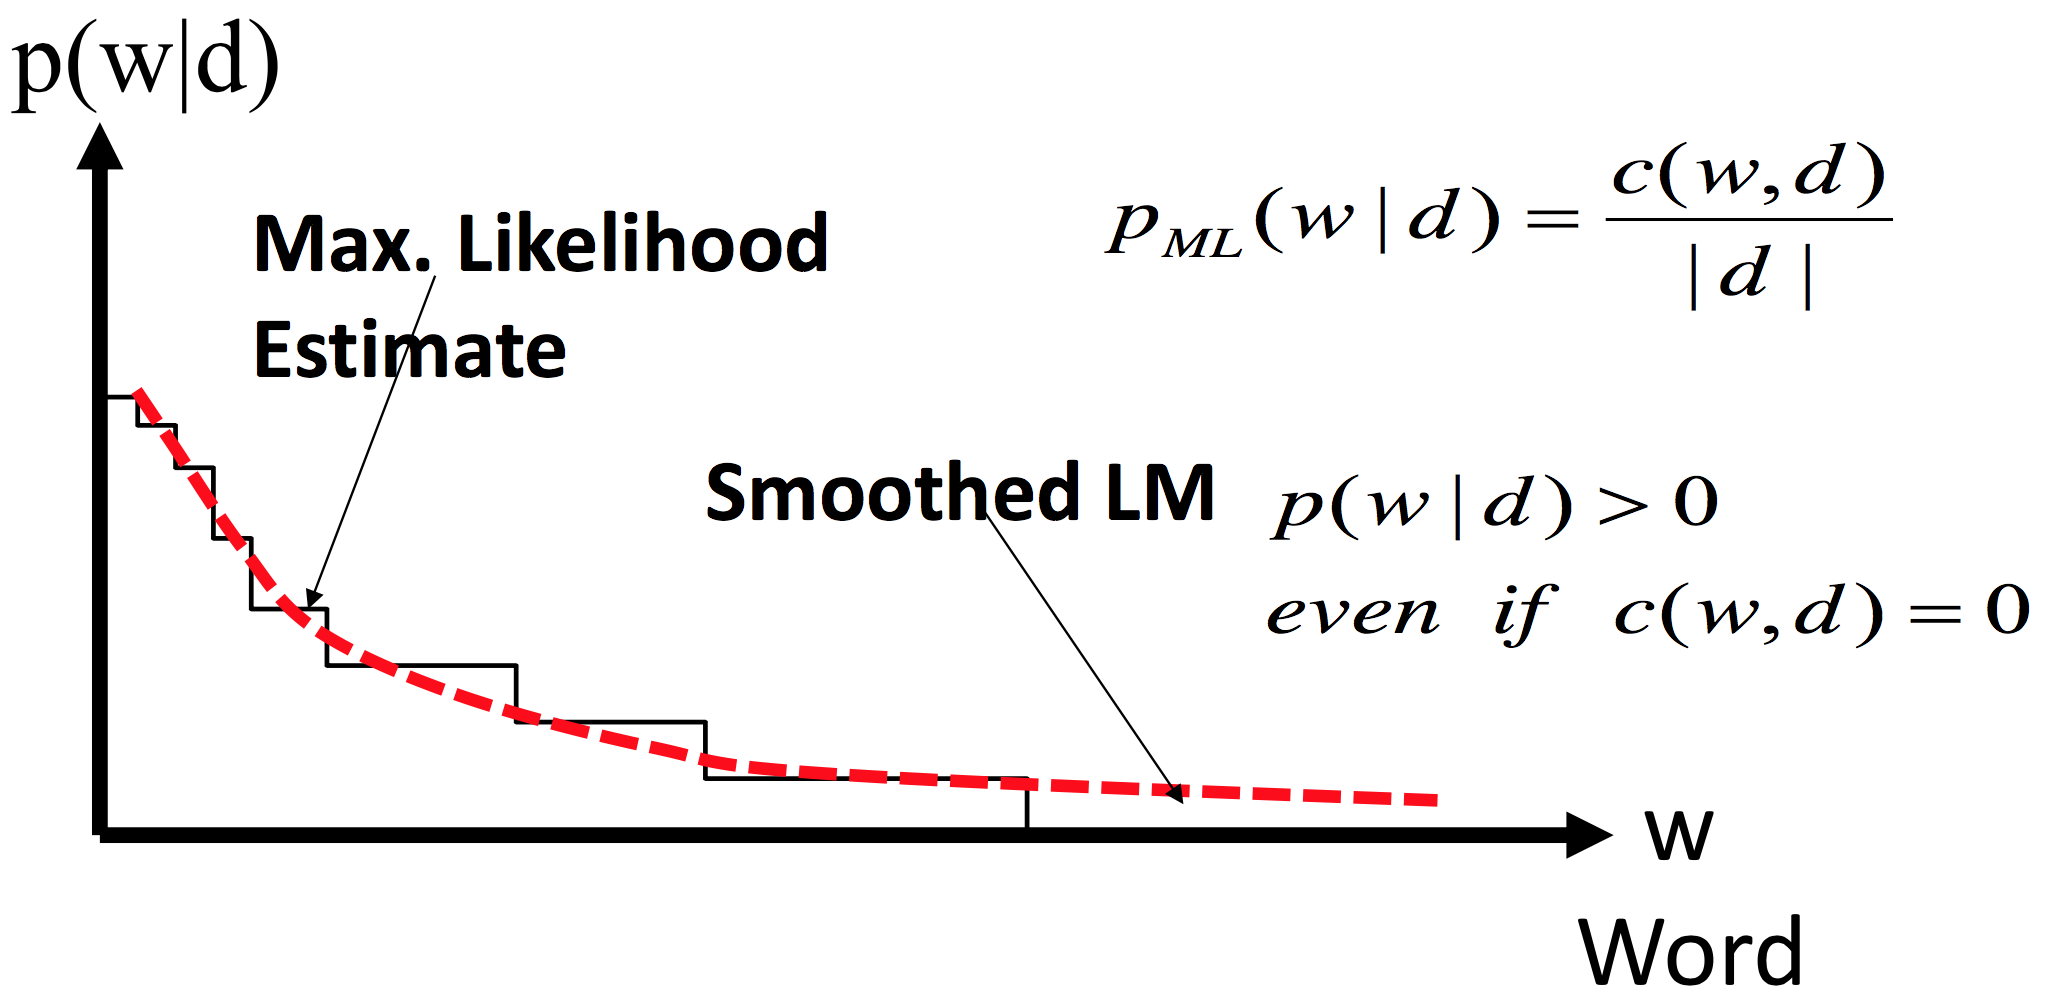
\includegraphics[width=0.7\linewidth]{smoothed_lm.png}
\end{figure}

Key Question: what probability should be assigned to an unseen word? Let the probability of an unseen word be proportional to its probability given by a reference LM. One possibility: Reference LM = Collection LM:
\begin{figure}[H]
    \centering
    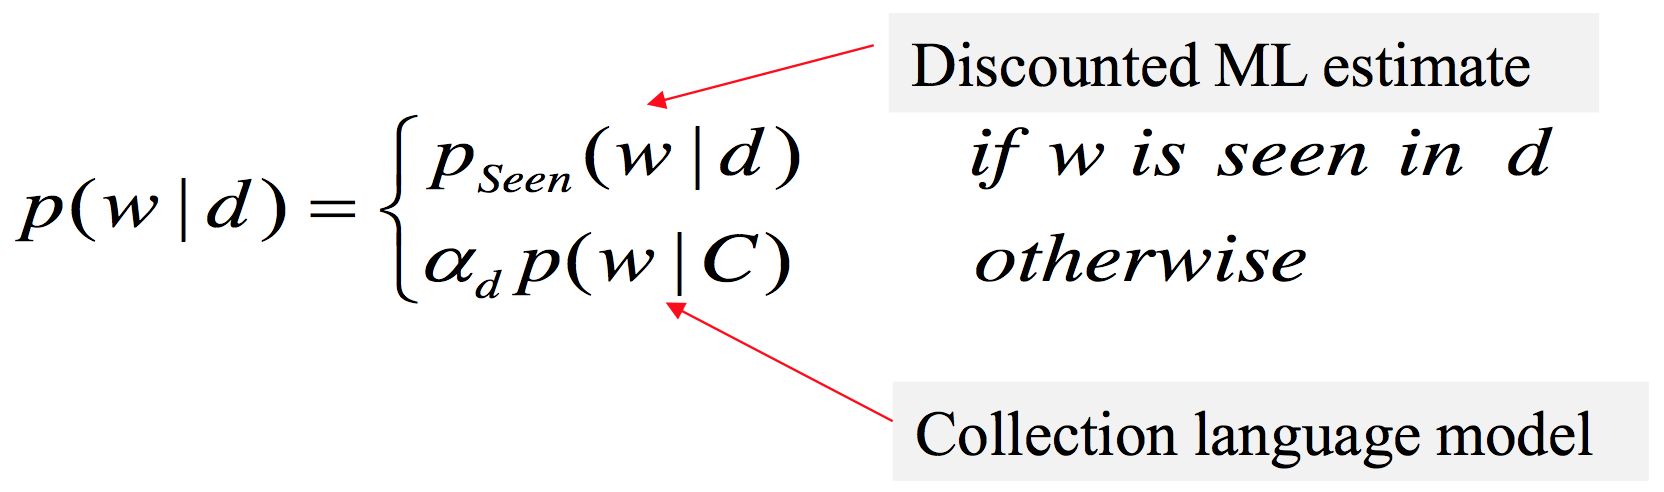
\includegraphics[width=0.6\linewidth]{probability_lm.png}
\end{figure}

%----------------------------------------
\subsection{Rewriting the Ranking Function with Smoothing}
\begin{figure}[H]
    \centering
    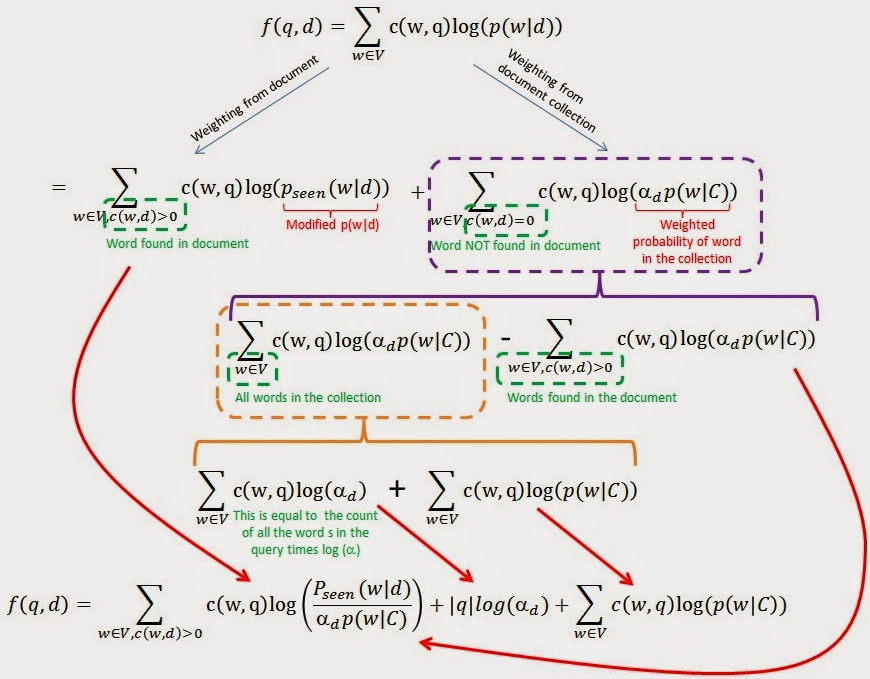
\includegraphics[width=\linewidth]{ranking_smoothing.png}
\end{figure}

%----------------------------------------
\subsection{Benefit of Rewriting}

Smoothing with $p(w \big| d)$ leads to a general ranking formula for query likelihood with TF- IDF weighting and document length normalization:
\begin{figure}[H]
    \centering
    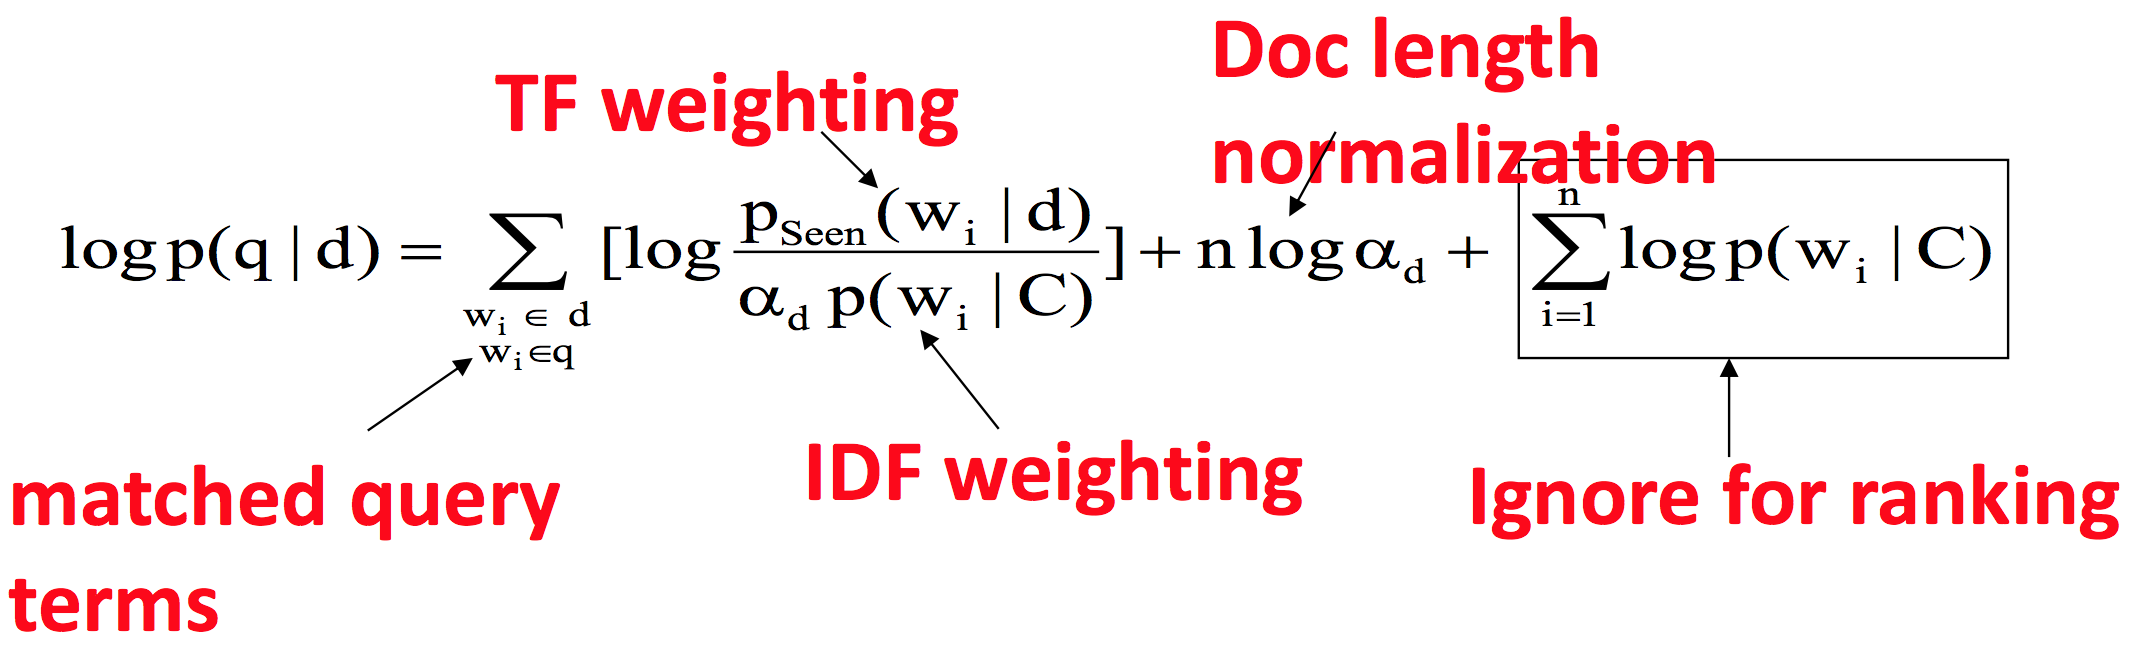
\includegraphics[width=0.8\linewidth]{ranking_smoothed.png}
\end{figure}

%----------------------------------------
\subsection{Smoothing Methods}
\begin{equation*}
f(q, d) = \sum_{w_i \in d, w_i \in q} c(w_i, q) \log \frac{p_{seen}(w_i \,\big|\, d)}{\alpha_d \, p(w_i \,\big|\, C)} + n \log \alpha_d
\end{equation*}

\subsubsection{Jelinek-Mercer Smoothing}
Jelinek-Mercer: Fixed coefficient linear interpolation
\begin{equation*}
p_{seen}(w \,\big|\, d) = (1-\lambda) \, \dfrac{c(w, d)}{|d|} + \lambda \, p(w \,\big|\, C), \quad \alpha_d = \lambda, \quad \lambda \in [0, 1]
\end{equation*}

Ranking Function:
\begin{equation*}
f_{JM}(q, d) = \sum_{w \in d, w \in q} c(w, q) \log \left( 1 + \frac{1-\lambda}{\lambda} \frac{c(w, d)}{|d| \, p(w \,\big|\, C)} \right)
\end{equation*}

\subsubsection{Dirichlet Prior (Bayesian) Smoothing}
Dirichlet Prior: Adding pseudo counts; adaptive interpolation
\begin{equation*}
p_{seen}(w \,\big|\, d) = \dfrac{c(w, d) + \mu \, p(w \,\big|\, C)}{|d| + \mu} = \dfrac{|d|}{|d| + \mu}\cdot\dfrac{c(w,d)}{|d|} + \dfrac{\mu}{|d| + \mu}\cdot p(w \,\big|\, C)
\end{equation*}

\begin{equation*}
\alpha_d = \frac{\mu}{|d| + \mu}, \quad \mu \in [0, +\infty)
\end{equation*}

Ranking Function:
\begin{equation*}
f_{DIR}(q, d) = \sum_{w \in d, w \in q} c(w, q) \log \left( 1 + \frac{c(w, d)}{\mu \, p(w \,\big|\, C)} \right) + n\,\log\frac{\mu}{\mu + |d|}
\end{equation*}

%----------------------------------------
\subsection{Summary of Query Likelihood Probabilistic Model}
\begin{itemize}
\item Effective ranking functions obtained using pure probabilistic modeling

\begin{itemize}
\item Assumption 1: $Relevance(q,d) = p(R=1 \,\big|\, q,d) \approx p(q \,\big|\, d,R=1) \approx p(q \,\big|\, d)$
\item Assumption 2: Query words are generated independently
\item Assumption 3: Smoothing with $p(w \,\big|\, C)$
\item Assumption 4: JM or Dirichlet prior smoothing
\end{itemize}

\item Less heuristic compared with VSM
\item Many extensions have been made [Zhai 08]
\end{itemize}

%----------------------------------------
\subsection{Recommended reading}
\begin{itemize}
\item ChengXiang Zhai, \href{http://www.morganclaypool.com/doi/abs/10.2200/S00158ED1V01Y200811HLT001}{<<Statistical Language Models for Information Retrieval>> (Synthesis Lectures Series on Human Language Technologies)}, Morgan \& Claypool Publishers, 2008.
\end{itemize}

